\documentclass[a4paper]{article}

\usepackage{Sweave} %--------------------------------!
\usepackage{amsmath}
\usepackage{amssymb}
\usepackage{amsthm}
\usepackage{fancyhdr}
\usepackage[usenames, dvipsnames]{color}
\usepackage{verbatim}

\oddsidemargin 0cm
\topmargin -2.4cm     %I recommend adding these three lines to increase the
\textwidth 16.5cm   %amount of usable space on the page (and save trees)
\textheight 27.5cm

\newcommand{\question}[2] {\vspace{.25in} \hrule\vspace{0.5em}
\noindent{\bf #1: #2} \vspace{0.5em}
\hrule \vspace{.10in}}
\renewcommand{\part}[1] {\vspace{.10in} {\bf (#1)}}

\newcommand{\myname}{Xuan Han}
\newcommand{\myhusky}{han.xua@husky.neu}
\newcommand{\myhwnum}{8}

\setlength{\parindent}{0pt}
\setlength{\parskip}{5pt plus 1pt}

\pagestyle{fancyplain}
\lhead{\fancyplain{}{\textbf{HW\myhwnum}}}      % Note the different brackets!
\rhead{\fancyplain{}{\myname\\ \myhusky}}
\chead{\fancyplain{}{1 2 3 4}}


\begin{document}
\Sconcordance{concordance:tree.tex:tree.Rnw:%
1 43 1 1 2 1 0 3 1 1 2 2 1 1 2 3 1 3 0 1 2 2 1 1 2 1 0 2 1 12 0 1 2 9 1 %
1 2 28 0 1 2 12 1 1 2 1 0 1 1 4 0 1 2 7 1 1 2 1 0 1 1 7 0 1 1 6 0 1 2 7 %
1 1 2 4 0 1 2 2 1 1 2 5 0 1 2 7 1 1 2 1 0 2 1 4 0 1 2 1 1 1 2 1 0 1 1 7 %
0 1 1 6 0 1 2 6 1 1 2 1 0 1 1 7 0 1 1 6 0 1 2 9 1 1 2 1 0 3 1 15 0 1 1 %
1 3 1 1 7 0 1 1 7 0 1 2 13 1 1 2 1 0 2 1 15 0 1 1 1 2 1 1 7 0 1 1 7 0 1 %
2 12 1 1 2 1 0 5 1 1 11 10 0 3 1 1 2 1 1 5 0 1 1 5 0 1 1 18 0 1 2 9 1}


\title{Data Mining Assignment \myhwnum}
\author{\myname \\
        \myhusky}
\date{\today}
\maketitle

\thispagestyle{plain}

\begin{Schunk}
\begin{Sinput}
> load('realEstate.RData')
> binQua = ifelse(realEstate$Quality == 1, 1, 0)
> binQua = as.factor(binQua)
> all.data = data.frame(realEstate, binQua)
> totalInstance = dim(realEstate)[1]
> trainSize = 350
> testSize = totalInstance - trainSize
> set.seed(1)
> trainIndex = sample(1:522, 350)
> trainSet = all.data[trainIndex, c(-1, -10)]
> validateSet = all.data[-trainIndex, c(-1, -10)]
\end{Sinput}
\end{Schunk}

\question{1}{Tree}
\part{b}
\begin{Schunk}
\begin{Sinput}
> library(tree)
> tree.realEstate = tree(binQua~., trainSet)
> summary(tree.realEstate)
\end{Sinput}
\begin{Soutput}
Classification tree:
tree(formula = binQua ~ ., data = trainSet)
Variables actually used in tree construction:
[1] "Sales"   "SqFeet"  "Year"    "LotSize"
Number of terminal nodes:  10 
Residual mean deviance:  0.09508 = 32.33 / 340 
Misclassification error rate: 0.02286 = 8 / 350 
\end{Soutput}
\end{Schunk}
{\color{red}
\begin{enumerate}
\item Training error rate is 0.02286.
\item There are 10 terminal nodes.
\item Training error changes everytime with different samples.
\end{enumerate}
}


\part{c}
\begin{Schunk}
\begin{Sinput}
> tree.realEstate
\end{Sinput}
\begin{Soutput}
node), split, n, deviance, yval, (yprob)
      * denotes terminal node

 1) root 350 294.200 0 ( 0.85143 0.14857 )  
   2) Sales < 364500 271  23.620 0 ( 0.99262 0.00738 )  
     4) Sales < 322500 248   0.000 0 ( 1.00000 0.00000 ) *
     5) Sales > 322500 23  13.590 0 ( 0.91304 0.08696 )  
      10) Sales < 335125 10  10.010 0 ( 0.80000 0.20000 ) *
      11) Sales > 335125 13   0.000 0 ( 1.00000 0.00000 ) *
   3) Sales > 364500 79 103.900 1 ( 0.36709 0.63291 )  
     6) Sales < 527875 48  64.440 0 ( 0.60417 0.39583 )  
      12) SqFeet < 3403.5 35  39.900 0 ( 0.74286 0.25714 )  
        24) Year < 1986.5 22   8.136 0 ( 0.95455 0.04545 )  
          48) LotSize < 21303 5   5.004 0 ( 0.80000 0.20000 ) *
          49) LotSize > 21303 17   0.000 0 ( 1.00000 0.00000 ) *
        25) Year > 1986.5 13  17.320 1 ( 0.38462 0.61538 )  
          50) LotSize < 22249 5   0.000 1 ( 0.00000 1.00000 ) *
          51) LotSize > 22249 8  10.590 0 ( 0.62500 0.37500 ) *
      13) SqFeet > 3403.5 13  14.050 1 ( 0.23077 0.76923 )  
        26) Sales < 458250 5   6.730 0 ( 0.60000 0.40000 ) *
        27) Sales > 458250 8   0.000 1 ( 0.00000 1.00000 ) *
     7) Sales > 527875 31   0.000 1 ( 0.00000 1.00000 ) *
\end{Soutput}
\end{Schunk}
{\color{red}
\begin{enumerate}
\item Let's look at node 2:
\item The split criterion is Sales < 322500
\item There are 271 data points in this node.
\item This terminal node label is 0.
\item Deviance is 23.62.
\item 0.99262 percent of the data points are labeled 0, and 0.00738 of the data points are labeled 1.
\end{enumerate}
}


\part{d}
\begin{Schunk}
\begin{Sinput}
> plot(tree.realEstate)
> text(tree.realEstate, pretty = 0)
\end{Sinput}
\end{Schunk}
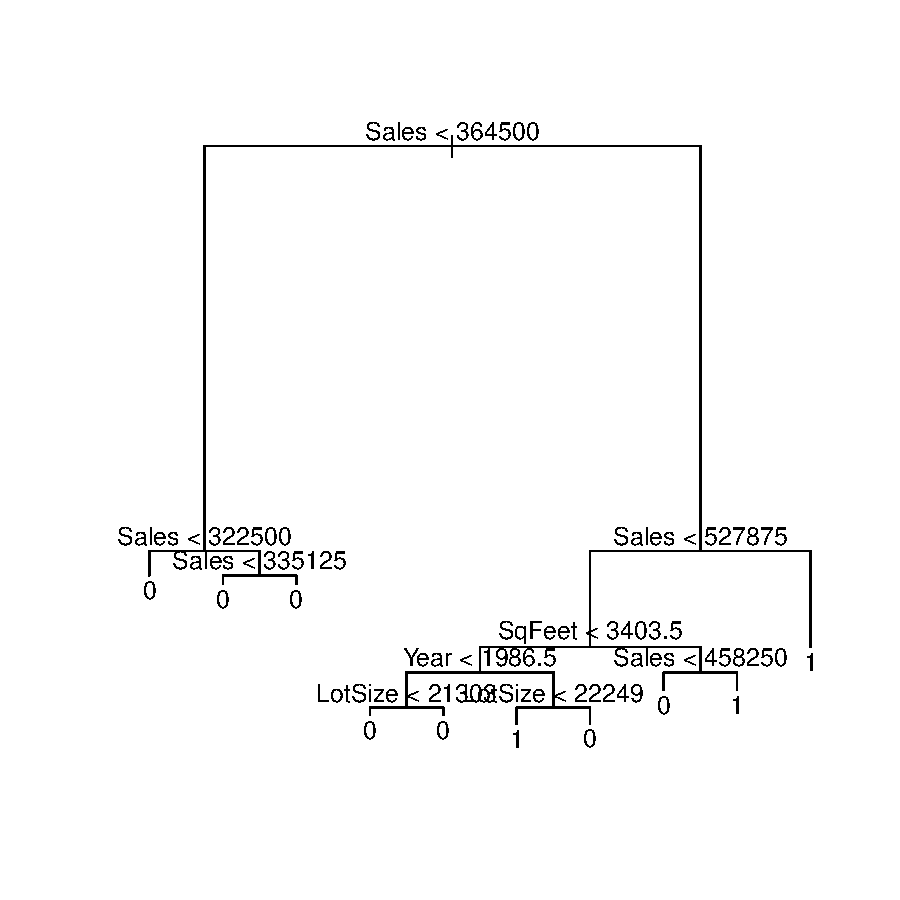
\includegraphics{tree-1d}
{\color{red}
\begin{enumerate}
\item This tree has depth 4.
\item The most important predictor is Sales. The first split differentiated most of the data points. And it appeared 5 times.
\end{enumerate}
}

\part{e}
\begin{Schunk}
\begin{Sinput}
> tree.pred = predict(tree.realEstate, validateSet, type = 'class')
> table(tree.pred, validateSet$binQua)
\end{Sinput}
\begin{Soutput}
tree.pred   0   1
        0 152   6
        1   4  10
\end{Soutput}
\begin{Sinput}
> (6 + 4) / 172
\end{Sinput}
\begin{Soutput}
[1] 0.05813953
\end{Soutput}
\end{Schunk}
{\color{red}
\begin{enumerate}
\item Test error rate is 0.05813953.
\end{enumerate}
}


\part{f}
\begin{Schunk}
\begin{Sinput}
> cv.realEstate = cv.tree(tree.realEstate, FUN = prune.misclass)
\end{Sinput}
\end{Schunk}


\part{g}
\begin{Schunk}
\begin{Sinput}
> plot(cv.realEstate$size, cv.realEstate$dev, type = 'b', col = 'red')
\end{Sinput}
\end{Schunk}
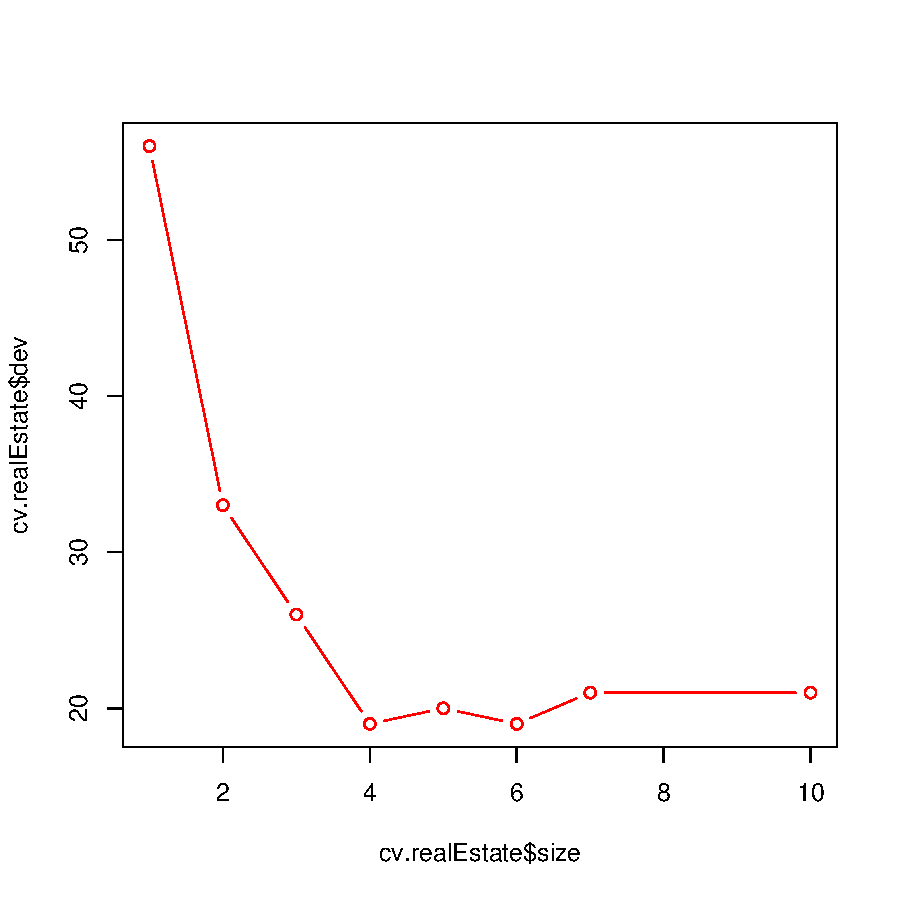
\includegraphics{tree-1g}
{\color{red}
\begin{enumerate}
\item As show in the plot, tree size 4 and 6 corresponding to the lowest cross-validated error rate.
\end{enumerate}
}


\part{h}
\begin{Schunk}
\begin{Sinput}
> prune.realEstate = prune.misclass(tree.realEstate, best = 6)
> plot(prune.realEstate)
> text(prune.realEstate, pretty = 0)
\end{Sinput}
\end{Schunk}
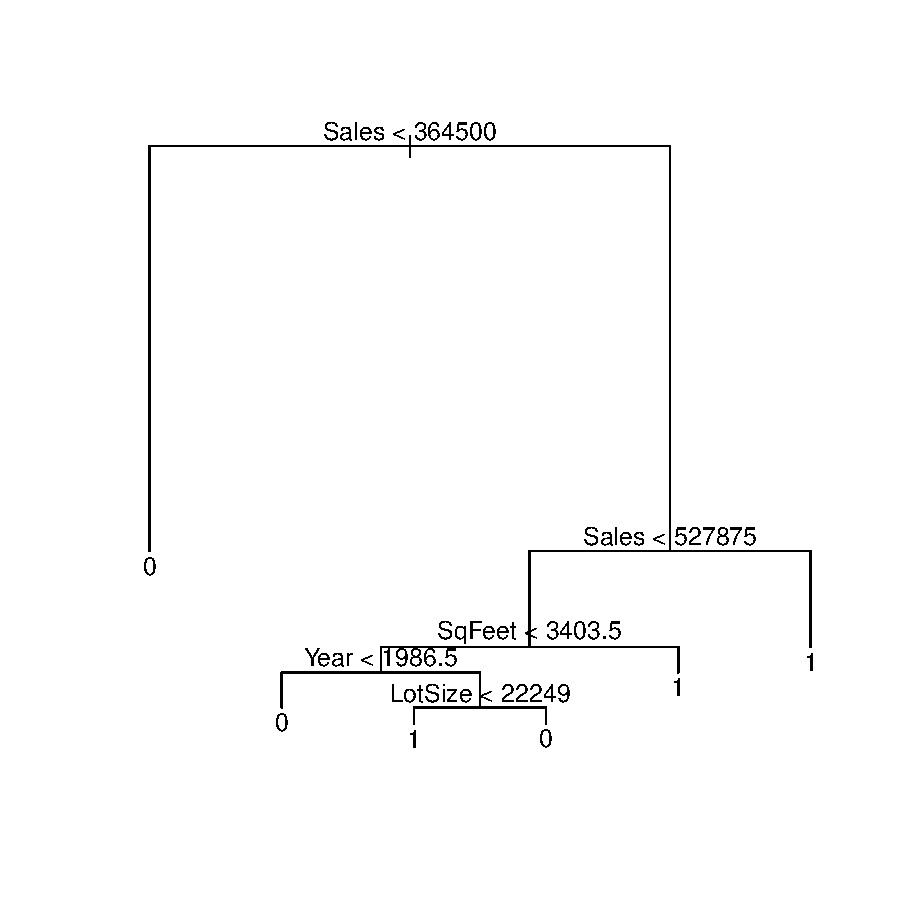
\includegraphics{tree-1h}

\part{j}
\begin{Schunk}
\begin{Sinput}
> prune.pred.train = predict(prune.realEstate, trainSet, type = 'class')
> table(prune.pred.train, trainSet$binQua)
\end{Sinput}
\begin{Soutput}
prune.pred.train   0   1
               0 295   6
               1   3  46
\end{Soutput}
\begin{Sinput}
> (6 + 3) / 350
\end{Sinput}
\begin{Soutput}
[1] 0.02571429
\end{Soutput}
\end{Schunk}
{\color{red}
\begin{enumerate}
\item Train error rate after prune if 0.0257, which is higher than unpruned tree.
\end{enumerate}
}

\part{k}
\begin{Schunk}
\begin{Sinput}
> prune.pred.validate = predict(prune.realEstate, validateSet, type = 'class')
> table(prune.pred.validate, validateSet$binQua)
\end{Sinput}
\begin{Soutput}
prune.pred.validate   0   1
                  0 148   5
                  1   8  11
\end{Soutput}
\begin{Sinput}
> (8 + 5) / 172
\end{Sinput}
\begin{Soutput}
[1] 0.0755814
\end{Soutput}
\end{Schunk}
{\color{red}
\begin{enumerate}
\item Test error rate after prune if 0.0755814, which is higher than unpruned tree.
\end{enumerate}
}



\newpage
\question{2}{Bagging}
\begin{Schunk}
\begin{Sinput}
> library(randomForest)
> set.seed(1)
> bag.realEstate = randomForest(binQua ~ ., data = trainSet, mtry = 11, importance = T, ntree = 100)
> bag.realEstate
\end{Sinput}
\begin{Soutput}
Call:
 randomForest(formula = binQua ~ ., data = trainSet, mtry = 11,      importance = T, ntree = 100) 
               Type of random forest: classification
                     Number of trees: 100
No. of variables tried at each split: 11

        OOB estimate of  error rate: 6.29%
Confusion matrix:
    0  1 class.error
0 289  9  0.03020134
1  13 39  0.25000000
\end{Soutput}
\begin{Sinput}
> varImpPlot(bag.realEstate, col = 'blue')
> yhat.bag = predict(bag.realEstate, newdata = validateSet)
> table(yhat.bag, validateSet$binQua)
\end{Sinput}
\begin{Soutput}
yhat.bag   0   1
       0 150   4
       1   6  12
\end{Soutput}
\begin{Sinput}
> (6 + 4) / 172
\end{Sinput}
\begin{Soutput}
[1] 0.05813953
\end{Soutput}
\end{Schunk}
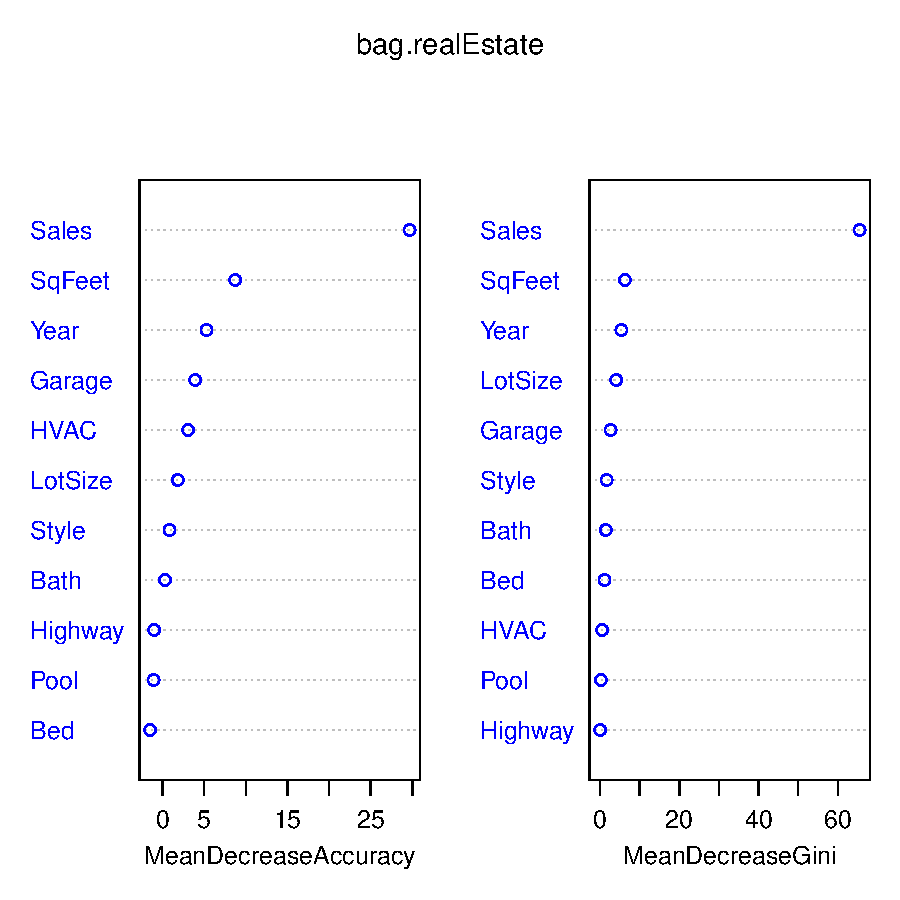
\includegraphics{tree-2}

{\color{red}
\begin{enumerate}
\item We can see that Sales is the most important predictor.
\item Train error rate is 0.0629, higher than the best single-tree classification.
\item Test error rate is 0.05813953, equal with the best single-tree classification.
\end{enumerate}
}



\newpage
\question{3}{RandomForest}

\begin{Schunk}
\begin{Sinput}
> set.seed(1)
> forest.realEstate = randomForest(binQua ~ ., data = trainSet, mtry = 1, importance = T, ntree = 100)
> forest.realEstate
\end{Sinput}
\begin{Soutput}
Call:
 randomForest(formula = binQua ~ ., data = trainSet, mtry = 1,      importance = T, ntree = 100) 
               Type of random forest: classification
                     Number of trees: 100
No. of variables tried at each split: 1

        OOB estimate of  error rate: 6.29%
Confusion matrix:
    0  1 class.error
0 295  3  0.01006711
1  19 33  0.36538462
\end{Soutput}
\begin{Sinput}
> varImpPlot(forest.realEstate, col = 'blue')
> yhat.forest = predict(forest.realEstate, newdata = validateSet)
> table(yhat.forest, validateSet$binQua)
\end{Sinput}
\begin{Soutput}
yhat.forest   0   1
          0 153   4
          1   3  12
\end{Soutput}
\begin{Sinput}
> (4 + 3) / 172
\end{Sinput}
\begin{Soutput}
[1] 0.04069767
\end{Soutput}
\end{Schunk}
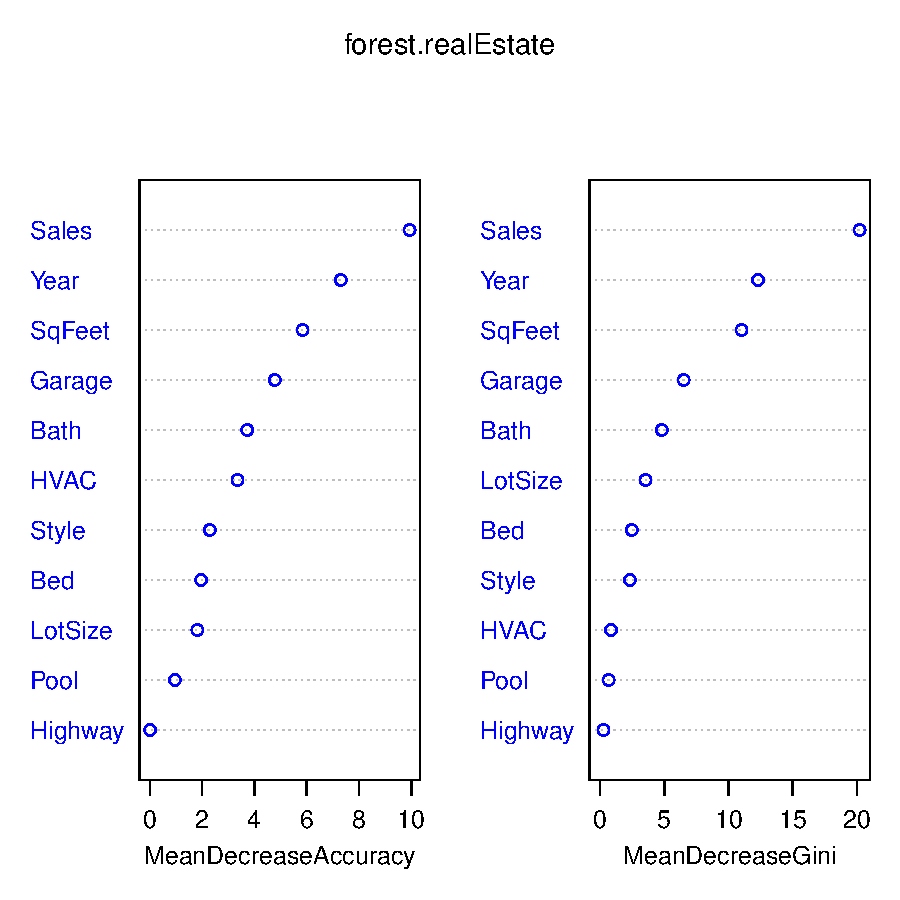
\includegraphics{tree-3}
{\color{red}
\begin{enumerate}
\item Train is 0.629, higher than best single tree.
\item Test error is 0.04069767, lower than best single tree.
\item Importance map changed a litter bit. Other variables have more infulence now, which is as expected.
\item Note that I set mtry = 1, which gives the best test error.
\end{enumerate}
}



\newpage
\question{4}{Boosting}

\begin{Schunk}
\begin{Sinput}
> require(gbm)
> set.seed(1)
> shirinkages = seq(from = 0, to = 0.6, by = 0.02)
> trainAccu = rep(NA, length(shirinkages))
> testAccu = rep(NA, length(shirinkages))
> counter = 1
> trainSet$binQua = as.numeric(trainSet$binQua) - 1
> validateSet$binQua = as.numeric(validateSet$binQua) - 1
> for (s in shirinkages) {
+     boost.realEstate = gbm(binQua ~ ., data = trainSet, distribution = "bernoulli", n.trees = 1000, shrinkage = s)
+     yhat.boost.vali.probs = predict(boost.realEstate, newdata = validateSet, n.trees = 1000, type = 'response')
+     yhat.boost.vali.preds = ifelse(yhat.boost.vali.probs > 0.5, 1, 0)
+     yhat.boost.train.probs = predict(boost.realEstate, newdata = trainSet, n.trees = 1000, type = 'response')
+     yhat.boost.train.preds = ifelse(yhat.boost.train.probs > 0.5, 1, 0)
+ 
+     trainAccu[counter] = sum(yhat.boost.train.preds == trainSet$binQua) / 350
+     testAccu[counter] = sum(yhat.boost.vali.preds == validateSet$binQua) / 172
+     counter = counter + 1
+ }
> par(mfrow = c(2, 2))
> plot(shirinkages, trainAccu, type = 'l')
> plot(shirinkages, testAccu, type = 'l')
> best = which.max(testAccu)
> 1 - testAccu[best]
\end{Sinput}
\begin{Soutput}
[1] 0.05232558
\end{Soutput}
\begin{Sinput}
> 1 - trainAccu[best]
\end{Sinput}
\begin{Soutput}
[1] 0
\end{Soutput}
\begin{Sinput}
> summary(boost.realEstate)
\end{Sinput}
\begin{Soutput}
            var      rel.inf
Sales     Sales 9.715107e+01
Year       Year 2.728681e+00
SqFeet   SqFeet 1.142591e-01
Bed         Bed 3.947412e-03
Garage   Garage 1.459663e-03
Style     Style 5.799144e-04
Bath       Bath 0.000000e+00
HVAC       HVAC 0.000000e+00
Pool       Pool 0.000000e+00
LotSize LotSize 0.000000e+00
Highway Highway 0.000000e+00
\end{Soutput}
\end{Schunk}
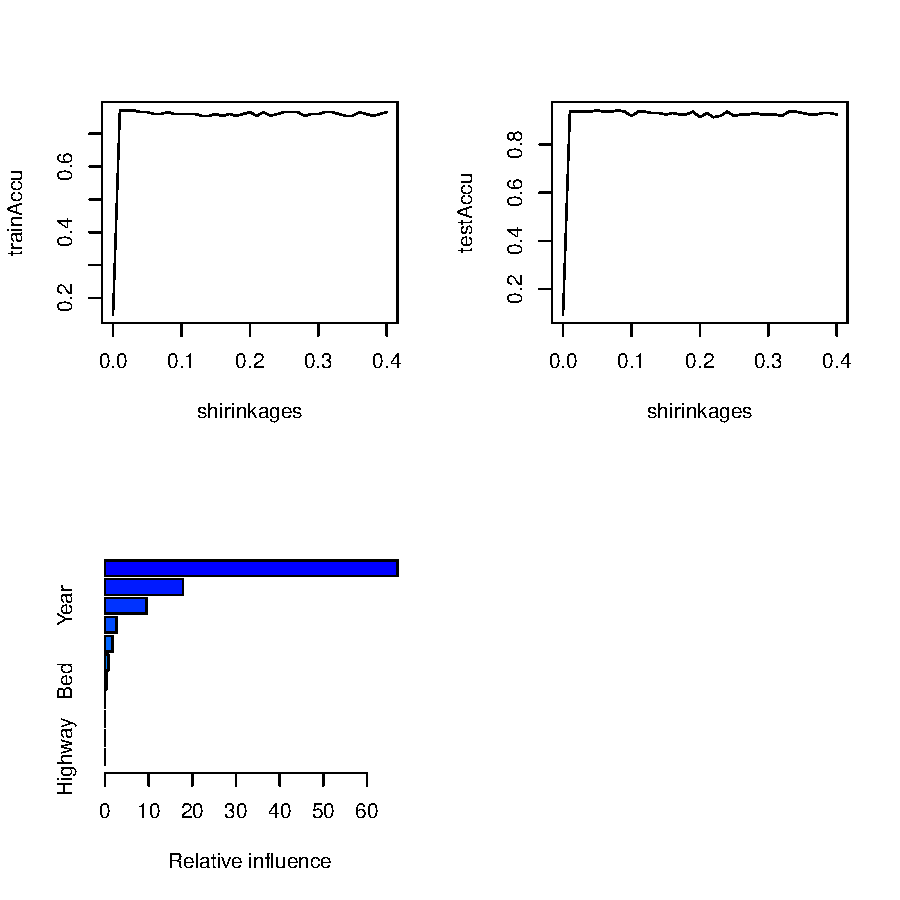
\includegraphics{tree-4}

{\color{red}
\begin{enumerate}
\item Test error rate is 0.05232558, lower than best single tree model.
\item Train error rate is 0, lower than best single tree.
\item The most important variable is Sales and Year
\end{enumerate}
}

\end{document}
